\section{研究方法}

本节详细介绍研究中采用的方法和技术路线,包括数据预处理、特征工程、模型选择等关键步骤\cite{hastie2009elements}。

\subsection{回归算法原理}
\subsubsection{回归分析基础}
回归分析是一种预测性建模技术,主要研究因变量(目标变量)和自变量(特征变量)之间的关系\cite{li2021comparative}。其基本假设包括:
\begin{itemize}
    \item 线性性:变量之间存在线性关系
    \item 独立性:观测值之间相互独立
    \item 同方差性:误差项具有相同的方差
    \item 正态性:误差项服从正态分布
\end{itemize}

\subsubsection{随机森林算法原理}
随机森林是一种集成学习方法,其核心原理包括:
\begin{enumerate}
    \item Bootstrap采样
    \begin{itemize}
        \item 从原始数据集中有放回抽样,构建多个子数据集
        \item 每个子数据集用于训练一个决策树
    \end{itemize}
    
    \item 决策树构建
    \begin{itemize}
        \item 在每个节点随机选择特征子集
        \item 使用最佳分裂特征进行节点分裂
        \item 直到达到停止条件(如最大深度)
    \end{itemize}
    
    \item 集成预测
    \begin{itemize}
        \item 对于回归问题,取所有树预测结果的平均值
        \item 降低过拟合风险,提高模型稳定性
    \end{itemize}
\end{enumerate}

\subsubsection{决策树算法原理}
决策树回归的基本原理:
\begin{enumerate}
    \item 特征选择
    \begin{itemize}
        \item 使用均方误差(MSE)作为分裂标准
        \item MSE = $\frac{1}{n}\sum_{i=1}^n(y_i - \bar{y})^2$
    \end{itemize}
    
    \item 树的生长
    \begin{itemize}
        \item 递归二分:选择最优分裂点
        \item 最小化子节点的均方误差
    \end{itemize}
    
    \item 剪枝策略
    \begin{itemize}
        \item 预剪枝:限制树的生长
        \item 后剪枝:移除不重要的子树
    \end{itemize}
\end{enumerate}

\subsubsection{支持向量回归(SVR)原理}
SVR的核心思想:
\begin{itemize}
    \item 引入$\varepsilon$-不敏感损失函数
    \item 构建最优化问题:
    \[ \min \frac{1}{2}\|w\|^2 + C\sum_{i=1}^n(\xi_i + \xi_i^*) \]
    \item 使用核函数处理非线性问题
    \item 通过对偶问题求解最优解
\end{itemize}

\subsubsection{神经网络回归原理}
神经网络回归模型的关键要素:
\begin{enumerate}
    \item 网络结构
    \begin{itemize}
        \item 输入层:特征变量
        \item 隐藏层:非线性变换
        \item 输出层:预测值
    \end{itemize}
    
    \item 激活函数
    \begin{itemize}
        \item ReLU: $f(x) = \max(0,x)$
        \item Sigmoid: $f(x) = \frac{1}{1+e^{-x}}$
        \item Tanh: $f(x) = \frac{e^x-e^{-x}}{e^x+e^{-x}}$
    \end{itemize}
    
    \item 损失函数
    \begin{itemize}
        \item 均方误差(MSE)
        \item 平均绝对误差(MAE)
        \item Huber损失
    \end{itemize}
    
    \item 优化算法
    \begin{itemize}
        \item 随机梯度下降(SGD)
        \item Adam优化器
        \item 学习率调整策略
    \end{itemize}
\end{enumerate}

\subsection{数据获取与预处理}
\subsubsection{数据集描述}
本研究使用的数据集来源于空气质量监测站的实际观测数据,包含了从2010年1月2日到2014年12月25日期间的35,746条小时级别的观测记录。数据集涵盖了多个维度的环境监测指标,包括气象观测数据(如温度、气压、风向等)和空气质量指标。为了保证数据质量,我们对原始数据进行了全面的预处理,包括缺失值处理、异常值检测和特征工程等步骤。在特征工程阶段,我们还构建了一些新的时间特征,如年份、月份、星期几等,以捕捉空气质量的时间模式和周期性变化。

数据集中的主要特征及其说明如下表所示:

\begin{table}[H]
    \centering
    \begin{tabular}{lll}
        \toprule
        特征名称 & 单位 & 说明 \\
        \midrule
        DEWP & 摄氏度 & 露点温度 \\
        Ir & 小时 & 累计降雨时长 \\
        Is & 小时 & 累计降雪时长 \\
        Iws & m/s & 风速 \\
        PRES & hPa & 气压 \\
        TEMP & 摄氏度 & 温度 \\
        cbwd & - & 风向(NE/NW/SE/cv)\\
        Label & - & 空气质量指数(AQI)\\
        \bottomrule
    \end{tabular}
    \caption{数据集特征说明}
    \label{tab:feature_description}
\end{table}

\subsubsection{数据预处理}
数据预处理主要包括以下步骤:
\begin{enumerate}
    \item 缺失值处理
    \item 异常值检测与处理
    \item 数据标准化
    \item 特征选择与工程
\end{enumerate}

\subsubsection{缺失值分析}
对数据集进行缺失值分析,结果如图\ref{fig:missing_values}所示。通过热力图可以直观地观察到各特征的缺失情况,这为后续的数据填补策略提供了重要依据。

\begin{figure}[H]
    \centering
    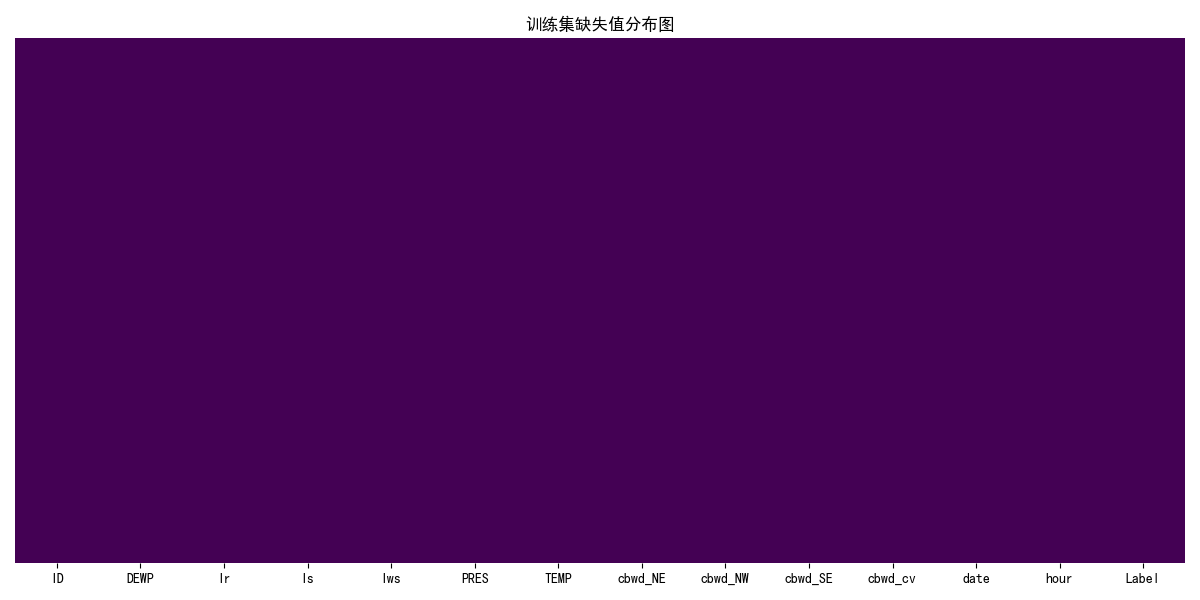
\includegraphics[width=0.8\textwidth]{images/missing_values_heatmap.png}
    \caption{特征缺失值分布热力图}
    \label{fig:missing_values}
\end{figure}

\subsubsection{异常值分析}
使用箱线图对数值型特征进行异常值检测,如图\ref{fig:outliers}所示。这种可视化方法帮助我们识别和处理数据中的异常点。

\begin{figure}[H]
    \centering
    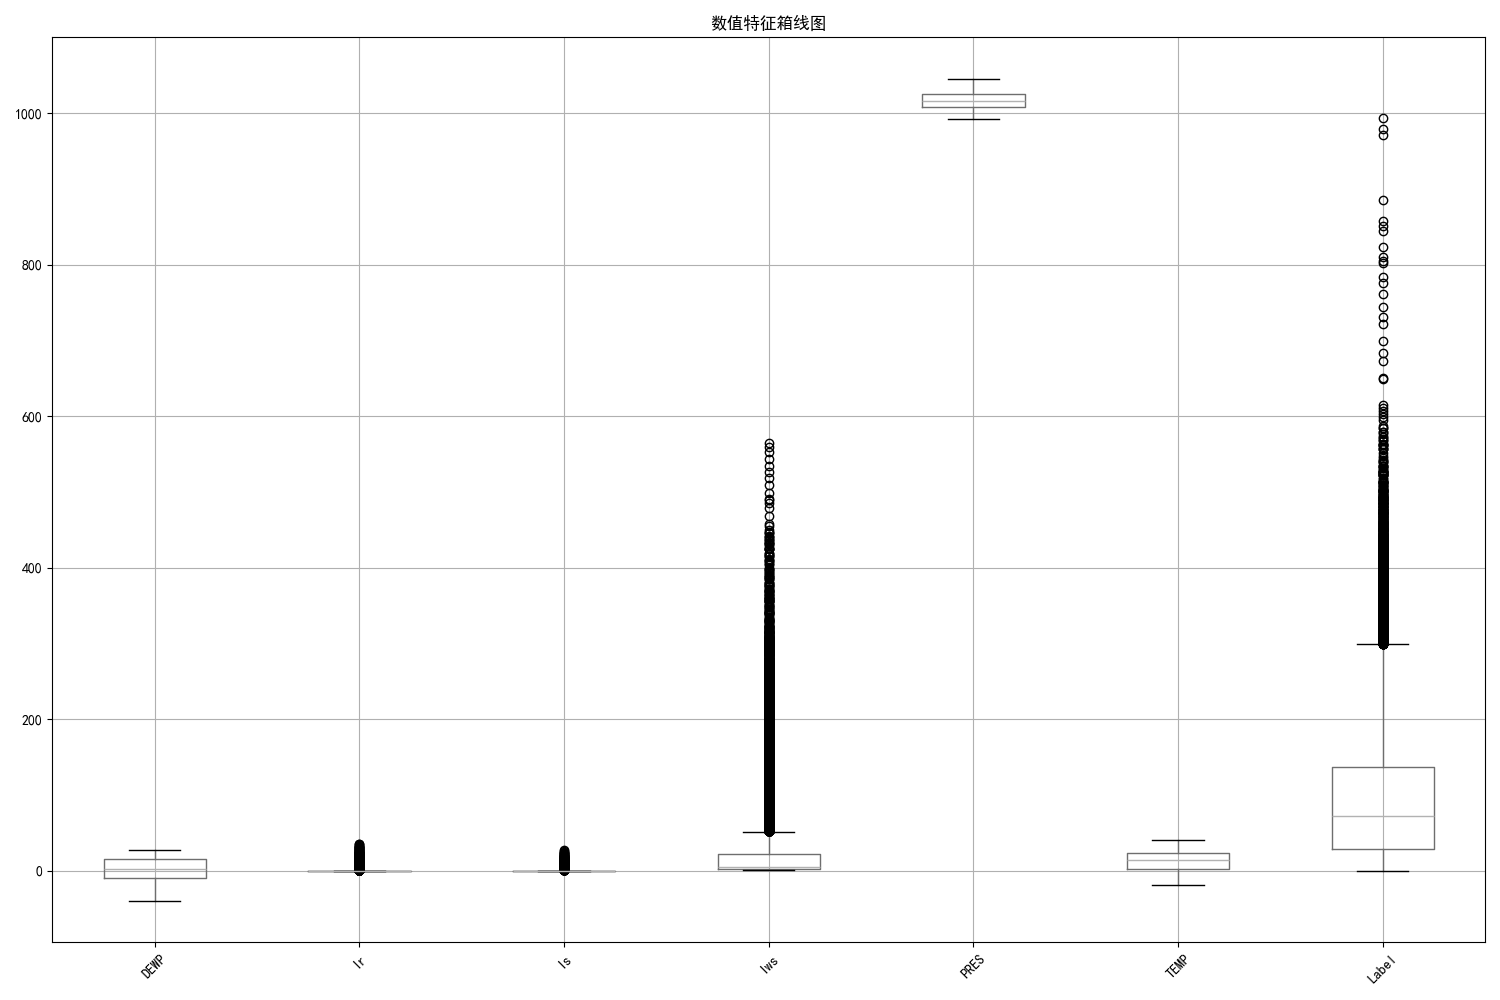
\includegraphics[width=0.8\textwidth]{images/outliers_boxplot.png}
    \caption{数值特征异常值箱线图}
    \label{fig:outliers}
\end{figure}

\subsection{特征工程与选择}
在特征工程阶段,我们综合考虑了多个维度的特征变量。首先是气象特征,包括温度、湿度、风向和风速等基础气象指标,这些因素直接影响着空气质量的变化。其次是时间特征,我们提取了年、月、日、小时等时间维度信息,用于捕捉空气质量的周期性变化规律。此外,我们还构建了一系列派生特征,如移动平均值和趋势指标等,这些特征能够反映空气质量的动态变化趋势。在特征选择过程中,我们采用了多种方法进行特征筛选和降维。通过相关性分析,我们识别并去除了高度相关的冗余特征;利用主成分分析(PCA)技术,我们降低了特征空间的维度,提取了最具代表性的特征组合;同时,我们还通过特征重要性评估,确定了对预测结果影响最显著的关键特征。

\subsection{模型构建与评估}
在模型选择方面,我们采用了多种主流的机器学习算法进行对比实验。随机森林模型凭借其优秀的集成学习能力,能够有效处理高维特征空间并降低过拟合风险;决策树模型提供了清晰的决策规则,具有较好的可解释性;支持向量机(SVM)在处理非线性关系方面表现出色;而神经网络模型则通过其强大的特征学习能力,能够捕捉数据中的复杂模式。在模型训练过程中,我们采用了严格的方法论:首先将数据集按7:2:1的比例划分为训练集、验证集和测试集,确保模型评估的客观性;然后通过网格搜索等方法对模型的超参数进行优化;同时使用k折交叉验证技术评估模型的稳定性;最后,我们还尝试了模型集成方法,进一步提升预测性能。

为了全面评估模型性能,我们采用了多个评估指标。均方根误差(RMSE)用于衡量预测值与真实值的偏差程度;平均绝对误差(MAE)提供了预测误差的直观度量;决定系数($R^2$)反映了模型对数据变异性的解释程度;预测准确率则直接反映了模型在实际应用中的表现。这些多维度的评估指标帮助我们全面理解模型的优势和局限性,为模型选择和优化提供了可靠的依据。

\subsubsection{软件环境}
\begin{itemize}
    \item 操作系统:Windows 11
    \item 编程语言:Python 3.12
    \item 主要库:scikit-learn, pandas, numpy, matplotlib, seaborn, plotly, xgboost, lightgbm, catboost
\end{itemize} 